\section{Methods}\label{sec:methods}
In this chapter we are clarifying the Loss and Metric Functions, the Architecture BERT used for our Experiments, Ideas principles like Adapter Tuning and
Sentence Embedding and how fusing different Dataset together works, which are used in training loop.


\subsection{BERT}
\begin{figure}[h]
    \centering
    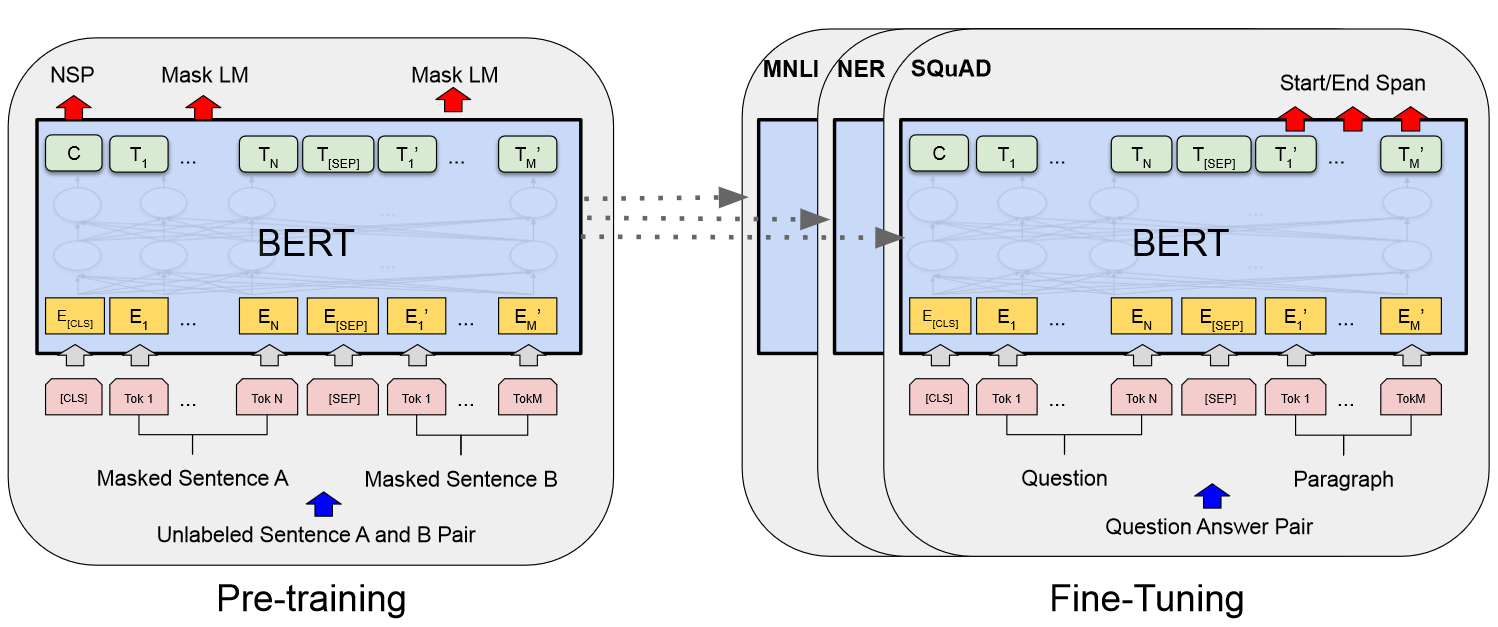
\includegraphics[scale=0.33]{./content/BERT_Architecture.png}
    \caption{Bidirectional Encoder Representations from Transformers (BERT) 
             scematic View \cite{devlin_bert_2019}.}
    \label{tab:bert}
\end{figure}

The Experiments are using BERT, Bidirectional Encoder Representations from Transformers (see Fig.~\ref{tab:bert}) ~\cite{devlin_bert_2019} 
developed by Google is based on Transformer architecture introduced by Vaswani et. al. \cite{vaswani_attention_2023}.
Unlike previous attempts, that process text in a unidirectional way (either left to right or right to 
left), BERT is designed to understand context bidirectionally as every Token is connected Pathways with every other. A masked language model (MLM) 
pre-training target is used, where tokens are randomly masked from the input to predict the original 
vocabulary IDs.
The model can be fine-tuned for specific downstream tasks, such as classification or translation. 
BERT is available in different sizes like BERT-Base and BERT-Large. There are various implementations 
such as RoBERTa~\cite{liu_roberta_2019}, ALBERT~\cite{lan_albert_2020}, BART~\cite{lewis_bart_2020}, 
DeBERTa~\cite{he_deberta_2021}, which improves BERT architecture differently.














\subsection{Sentence Embedding Architectures}
\textcolor{red}{TODO}

















\subsection{Adapter Tuning}
\begin{figure}[h]
    \centering
    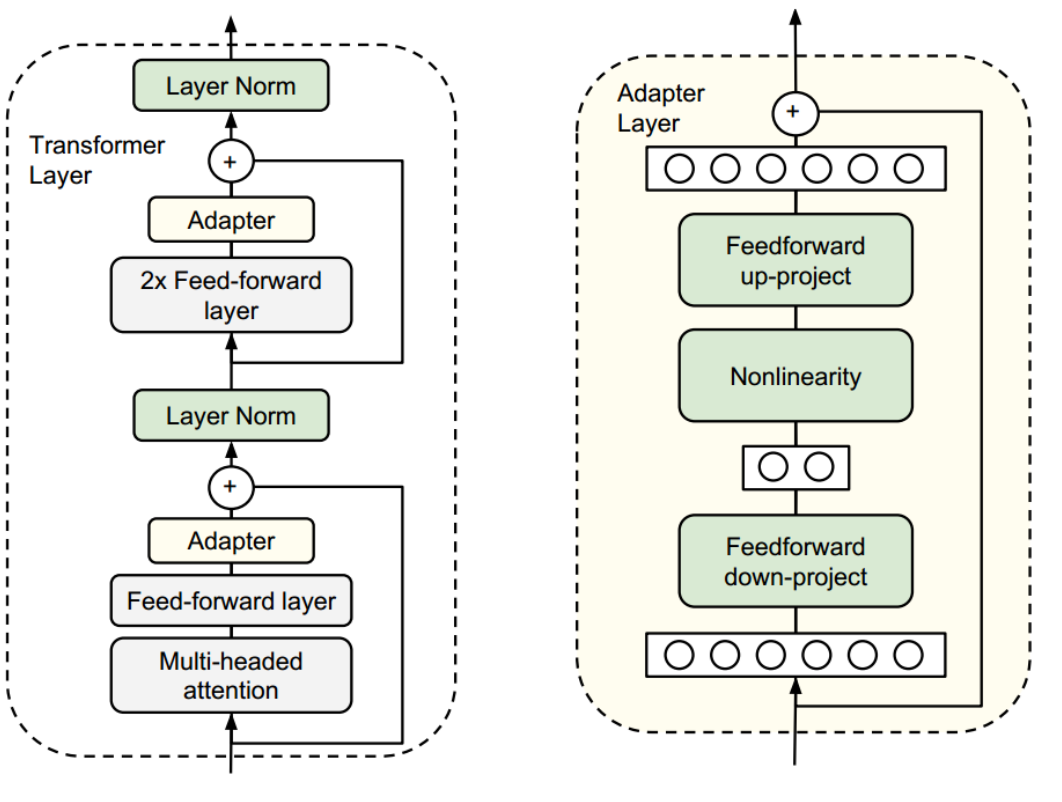
\includegraphics[scale=0.2]{./content/Adapter_Architecture.png}
    \caption{Basic Structure of Adapter built on top of a Models Architecture, where only the Adapter Layers Parameters are trainable \cite{zheng_learn_2023}.}
    \label{tab:bert}
\end{figure}

Adapter Tuning is a supervised method, where input, gold label are given and the models parameters are frozen, 
but adding new fully trainable bottleneck feed-forward networks 
on each intermediate layer. The objective is to reduce the size of trainable parameters, 
to gain higher throughput and keeping the pre-trained embeddings\cite{zheng_learn_2023} \cite{naveed_comprehensive_2023}. 
The ultimate goal of adaptation training is to enhance the model's scores on the downstream task, 
while still benefiting from the broad language understanding gained during the initial 
pre-training \cite{manjavacas_adapting_2022}. The effectiveness of adaptation-tuning depends on 
the similarity between the pre-training task and the target task due to fixed embeddings.













\subsection{Fusing different Datasets/Loaders}
\begin{figure}[h]
    \centering
    \resizebox{\textwidth}{!}{\begin{tikzpicture}
	\begin{pgfonlayer}{nodelayer}
		\node [style=base] (0) at (0, 0) {};
		\node [style=1x1 v1] (1) at (-7.5, 0) {};
		\node [style=1x1 v1] (4) at (-6.5, 0) {};
		\node [style=1x1 v1] (6) at (-5.5, 0) {};
		\node [style=1x1 v1] (7) at (-4.5, 0) {};
		\node [style=1x1 v3] (9) at (-3.5, 0) {};
		\node [style=1x1 v3] (10) at (-2.5, 0) {};
		\node [style=1x1 v3] (11) at (-1.5, 0) {};
		\node [style=1x1 v3] (12) at (-0.5, 0) {};
		\node [style=1x1 v4] (35) at (0.5, 0) {};
		\node [style=1x1 v4] (36) at (1.5, 0) {};
		\node [style=1x1 v4] (37) at (2.5, 0) {};
		\node [style=1x1 v4] (38) at (3.5, 0) {};
		\node [style=1x1 v2] (39) at (4.5, 0) {};
		\node [style=1x1 v2] (40) at (5.5, 0) {};
		\node [style=1x1 v2] (41) at (6.5, 0) {};
		\node [style=1x1 v2] (42) at (7.5, 0) {};
		\node [style=base] (43) at (19, 0) {};
		\node [style=1x1 v1] (44) at (11.5, 0) {};
		\node [style=1x1 v1] (45) at (12.5, 0) {};
		\node [style=1x1 v1] (46) at (13.5, 0) {};
		\node [style=1x1 v1] (47) at (14.5, 0) {};
		\node [style=1x1 v3] (48) at (15.5, 0) {};
		\node [style=1x1 v3] (49) at (16.5, 0) {};
		\node [style=1x1 v4] (52) at (17.5, 0) {};
		\node [style=1x1 v2] (56) at (19.5, 0) {};
		\node [style=1x1 v2] (57) at (24.5, 0) {};
		\node [style=1x1 v2] (58) at (25.5, 0) {};
		\node [style=1x1 v2] (59) at (26.5, 0) {};
		\node [style=base] (60) at (0, -3) {};
		\node [style=1x1 v1] (61) at (-7.5, -3) {};
		\node [style=1x1 v1] (62) at (-6.5, -3) {};
		\node [style=1x1 v1] (63) at (-5.5, -3) {};
		\node [style=1x1 v1] (64) at (-4.5, -3) {};
		\node [style=1x1 v3] (65) at (-3.5, -3) {};
		\node [style=1x1 v3] (66) at (-2.5, -3) {};
		\node [style=1x1 v3] (67) at (-1.5, -3) {};
		\node [style=1x1 v3] (68) at (-0.5, -3) {};
		\node [style=1x1 v4] (69) at (0.5, -3) {};
		\node [style=1x1 v4] (70) at (1.5, -3) {};
		\node [style=1x1 v4] (71) at (2.5, -3) {};
		\node [style=1x1 v4] (72) at (3.5, -3) {};
		\node [style=1x1 v2] (73) at (4.5, -3) {};
		\node [style=1x1 v2] (74) at (5.5, -3) {};
		\node [style=1x1 v2] (75) at (6.5, -3) {};
		\node [style=1x1 v2] (76) at (7.5, -3) {};
		\node [style=base] (77) at (0, -1.5) {};
		\node [style=1x1 v1] (78) at (-7.5, -1.5) {};
		\node [style=1x1 v1] (79) at (-6.5, -1.5) {};
		\node [style=1x1 v1] (80) at (-5.5, -1.5) {};
		\node [style=1x1 v1] (81) at (-4.5, -1.5) {};
		\node [style=1x1 v3] (82) at (-3.5, -1.5) {};
		\node [style=1x1 v3] (83) at (-2.5, -1.5) {};
		\node [style=1x1 v3] (84) at (-1.5, -1.5) {};
		\node [style=1x1 v3] (85) at (-0.5, -1.5) {};
		\node [style=1x1 v4] (86) at (0.5, -1.5) {};
		\node [style=1x1 v4] (87) at (1.5, -1.5) {};
		\node [style=1x1 v4] (88) at (2.5, -1.5) {};
		\node [style=1x1 v4] (89) at (3.5, -1.5) {};
		\node [style=1x1 v2] (90) at (4.5, -1.5) {};
		\node [style=1x1 v2] (91) at (5.5, -1.5) {};
		\node [style=1x1 v2] (92) at (6.5, -1.5) {};
		\node [style=1x1 v2] (93) at (7.5, -1.5) {};
		\node [style=base] (94) at (0, -4.5) {};
		\node [style=1x1 v1] (95) at (-7.5, -4.5) {};
		\node [style=1x1 v1] (96) at (-6.5, -4.5) {};
		\node [style=1x1 v1] (97) at (-5.5, -4.5) {};
		\node [style=1x1 v1] (98) at (-4.5, -4.5) {};
		\node [style=1x1 v3] (99) at (-3.5, -4.5) {};
		\node [style=1x1 v3] (100) at (-2.5, -4.5) {};
		\node [style=1x1 v3] (101) at (-1.5, -4.5) {};
		\node [style=1x1 v3] (102) at (-0.5, -4.5) {};
		\node [style=1x1 v4] (103) at (0.5, -4.5) {};
		\node [style=1x1 v4] (104) at (1.5, -4.5) {};
		\node [style=1x1 v4] (105) at (2.5, -4.5) {};
		\node [style=1x1 v4] (106) at (3.5, -4.5) {};
		\node [style=1x1 v2] (107) at (4.5, -4.5) {};
		\node [style=1x1 v2] (108) at (5.5, -4.5) {};
		\node [style=1x1 v2] (109) at (6.5, -4.5) {};
		\node [style=1x1 v2] (110) at (7.5, -4.5) {};
		\node [style=1x1 v1] (111) at (20.5, 0) {};
		\node [style=1x1 v1] (112) at (21.5, 0) {};
		\node [style=1x1 v3] (113) at (22.5, 0) {};
		\node [style=1x1 v2] (114) at (18.5, 0) {};
		\node [style=1x1 v4] (127) at (23.5, 0) {};
		\node [style=base] (128) at (19, -1.5) {};
		\node [style=1x1 v1] (129) at (11.5, -1.5) {};
		\node [style=1x1 v1] (130) at (12.5, -1.5) {};
		\node [style=1x1 v1] (131) at (13.5, -1.5) {};
		\node [style=1x1 v1] (132) at (14.5, -1.5) {};
		\node [style=1x1 v1] (140) at (20.5, -1.5) {};
		\node [style=1x1 v1] (141) at (21.5, -1.5) {};
		\node [style=1x1 v4] (144) at (19.5, -1.5) {};
		\node [style=1x1 v1] (145) at (15.5, -1.5) {};
		\node [style=1x1 v1] (146) at (16.5, -1.5) {};
		\node [style=1x1 v1] (147) at (17.5, -1.5) {};
		\node [style=1x1 v1] (148) at (18.5, -1.5) {};
		\node [style=1x1 v1] (149) at (22.5, -1.5) {};
		\node [style=1x1 v1] (150) at (23.5, -1.5) {};
		\node [style=1x1 v1] (151) at (24.5, -1.5) {};
		\node [style=1x1 v1] (152) at (25.5, -1.5) {};
		\node [style=1x1 v1] (153) at (26.5, -1.5) {};
		\node [style=base] (154) at (19, -3) {};
		\node [style=1x1 v1] (155) at (15.5, -3) {};
		\node [style=1x1 v1] (159) at (20.5, -3) {};
		\node [style=1x1 v1] (160) at (21.5, -3) {};
		\node [style=1x1 v4] (161) at (19.5, -3) {};
		\node [style=1x1 v1] (165) at (18.5, -3) {};
		\node [style=1x1 v1] (166) at (22.5, -3) {};
		\node [style=1x1 v1] (167) at (23.5, -3) {};
		\node [style=1x1 v1] (168) at (24.5, -3) {};
		\node [style=1x1 v1] (170) at (26.5, -3) {};
		\node [style=1x1 v4] (171) at (11.5, -3) {};
		\node [style=1x1 v4] (172) at (25.5, -3) {};
		\node [style=1x1 v4] (173) at (14.5, -3) {};
		\node [style=1x1 v3] (174) at (12.5, -3) {};
		\node [style=1x1 v2] (175) at (13.5, -3) {};
		\node [style=1x1 v2] (176) at (16.5, -3) {};
		\node [style=1x1 v2] (177) at (17.5, -3) {};
		\node [style=base] (178) at (19, -4.5) {};
		\node [style=1x1 v4] (182) at (19.5, -4.5) {};
		\node [style=1x1 v1] (183) at (18.5, -4.5) {};
		\node [style=1x1 v1] (185) at (23.5, -4.5) {};
		\node [style=1x1 v1] (186) at (24.5, -4.5) {};
		\node [style=1x1 v1] (187) at (26.5, -4.5) {};
		\node [style=1x1 v4] (188) at (12.5, -4.5) {};
		\node [style=1x1 v4] (189) at (25.5, -4.5) {};
		\node [style=1x1 v3] (191) at (11.5, -4.5) {};
		\node [style=1x1 v2] (192) at (13.5, -4.5) {};
		\node [style=1x1 v2] (193) at (16.5, -4.5) {};
		\node [style=1x1 v2] (194) at (17.5, -4.5) {};
		\node [style=1x1 v2] (195) at (14.5, -4.5) {};
		\node [style=1x1 v2] (196) at (15.5, -4.5) {};
		\node [style=1x1 v2] (197) at (20.5, -4.5) {};
		\node [style=1x1 v2] (198) at (21.5, -4.5) {};
		\node [style=1x1 v3] (199) at (22.5, -4.5) {};
		\node [style=Textfeld] (200) at (19, 1.25) {Combined Dataset};
		\node [style=Textfeld] (201) at (0, 1.25) {Combined Loader};
		\node [style=Textfeld] (202) at (9.5, 1.25) {Batch};
		\node [style=Textfeld] (203) at (9.5, 0) {1};
		\node [style=Textfeld] (204) at (9.5, -1.5) {2};
		\node [style=Textfeld] (205) at (9.5, -3) {...};
		\node [style=Textfeld] (206) at (9.5, -4.5) {n};
	\end{pgfonlayer}
\end{tikzpicture}
}
    \caption{Combined Dataset and Combined Loader Strategy where 4 different Dataset are getting mixed together.
             On the Loader-Level for a Batch size of 16, every Dataset is present equally and on the
             Dataset-Level, they are concatenated and the mixed.}\label{fig:test}
\end{figure}
Normally a Pre-Trained Model is used which is then fine-tuned on the Specific Dataset. The same can be applied to
Text Classification. Therefore the Model is performing only on SemEval very good, while mismatching on generalization
on other Text Classification Tasks. To Compensate, two strategies are applied to solve this.
CombinedLoaders is a strategy, where each Dataset, on which the Model should perform, can contribute equally with
the same amount of Datapoints. Another strategy involves the concatenation of all these Datasets to one and then being
mixed on the Training. For our Example (see Chapter~\ref{ch:ds}) we are using SNLI \cite{noauthor_snli_2023}
which has short sencences for entailment check, Healthver \cite{noauthor_dwaddenhealthver_entailment_nodate} a Dataset on the medical domain and
scifact \cite{noauthor_allenaiscifact_entailment_nodate} on the scientific domain, to check the entailment of claim, 
paper title and abstract. The Evaluation of the Strategies is only applied to SemEval Task Development
Dataset not on the choosen ones for expanding. Also the expected outcome should be lower than the
specialized Model on SemEval as it has to generalize the different domains more.























\subsection{Loss Functions and Evaluation Metric}
We are using 3 commonly used Loss functions for our Training of the different
Architectures with $x$ being the Prediction and $y$ being the searched Class. For direct Classification, 
CrossEntropyLoss~\ref{eq:ce} is the commonly and most frequently used function. Secondly, as we see later,
combined with Cosine Simmilarity, we are using MSELoss~\ref{eq:mse} or CosineEmbeddingLoss~\ref{eq:ceb}
to maximize or minimize the distance between two representations. As Metric the SemEval Task uses F1 Score, which
is the harmonic mean between precision and recall defined in Equation~\ref{eq:f} \cite{noauthor_nli4ct_nodate}.



\begin{equation}\label{eq:ce}
   Loss_{CE} = -\sum_{i=1}^My_{o,i}\log(x_{o,i})
\end{equation}
\begin{equation}\label{eq:mse}
   Loss_{MSE} = \sum_{i=1}^{M}(x_i-y_i)^2
\end{equation}

\begin{equation}\label{eq:ceb}
    Loss_{CEB} = \begin{cases}
        1 - \cos(x_1, x_2),      &\text{if $y = +1$}\\
        \max(0, \cos(x_1, x_2)), &\text{if $y = -1$}
    \end{cases}
\end{equation}

\begin{equation}\label{eq:f}
    F_1 = 2 \frac{precision \cdot recall}{precision + recall} = \frac{2 TP}{2TP + FP + FN}
 \end{equation}


